% Created 2024-07-15 Mon 01:45
% Intended LaTeX compiler: xelatex
\documentclass[a4paper,11pt,twoside]{article}
\usepackage{graphicx}
\usepackage{longtable}
\usepackage{wrapfig}
\usepackage{rotating}
\usepackage[normalem]{ulem}
\usepackage{amsmath}
\usepackage{amssymb}
\usepackage{capt-of}
\usepackage{hyperref}
\usepackage{libertine} \usepackage{amsmath}
\usepackage[width=200.00mm, height=240.00mm, left=3cm, right=3cm, top=3 cm, bottom=3cm]{geometry}
\usepackage{graphicx}
\graphicspath{ {./images/} }
\usepackage{multicol}
\author{Ryan P. Lynch}
\date{\today}
\title{Program 2A}
\hypersetup{
 pdfauthor={Ryan P. Lynch},
 pdftitle={Program 2A},
 pdfkeywords={},
 pdfsubject={},
 pdfcreator={Emacs 29.3 (Org mode 9.6.24)}, 
 pdflang={English}}
\usepackage{biblatex}

\begin{document}

\maketitle

\section*{Illustration of Stack}
\label{sec:org5f53a83}
\subsection*{Stack During func3 Looping}
\label{sec:orgdbb2187}
Starting state of the stack as laid out by the question.
\begin{center}
\begin{tabular}{ll}
\hline
\textbf{func3} & \emph{running}\\[0pt]
 & i = 4\\[0pt]
\hline
\textbf{func2} & \emph{waiting}\\[0pt]
 & i = 4\\[0pt]
\hline
\textbf{func1} & \emph{waiting}\\[0pt]
 & i = 4\\[0pt]
\hline
\textbf{main} & \emph{waiting}\\[0pt]
\hline
\end{tabular}
\end{center}

\subsection*{Stack After func3 Interrupt}
\label{sec:org95e0abc}
The time quantum of 5 seconds has passed. Therefore the alarm flag has been raised and a context change is performed by the scheduler.
\begin{center}
\begin{tabular}{ll}
\hline
\textbf{func3} & \emph{waiting}\\[0pt]
 & i = 4\\[0pt]
\hline
\textbf{func2} & \emph{waiting}\\[0pt]
 & i = 4\\[0pt]
\hline
\textbf{func1} & \emph{running}\\[0pt]
 & i = 5\\[0pt]
\hline
\textbf{main} & \emph{waiting}\\[0pt]
\hline
\end{tabular}
\end{center}
The scheduler picks \textbf{func1} to be executed. It does this because \textbf{func1} is at the front of the thread queue. This is true because it was the first to be added during the calling of \emph{sthread\textsubscript{create}} and the subsequent calling of \emph{capture} in \emph{sthread\textsubscript{init}}.
\pagebreak
\section*{Compile and Execution}
\label{sec:org38754b0}
\begin{multicols}{2}
\noindent
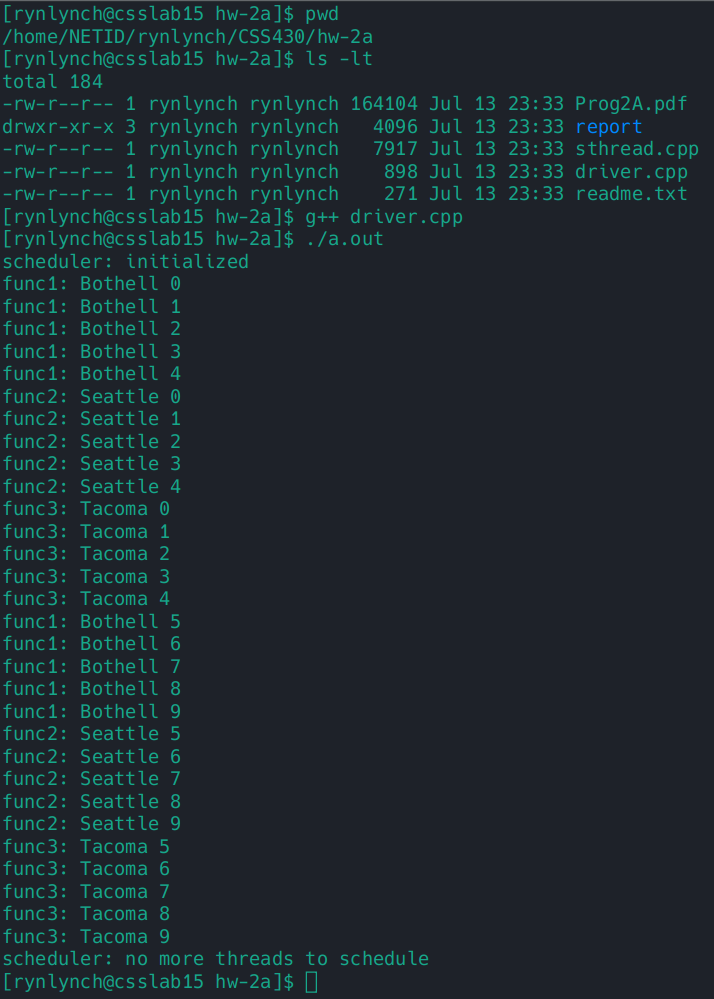
\includegraphics[width=0.5\textwidth]{compile-execution}
\vfill\null
\columnbreak
\noindent
The screenshot to the left shows driver.cpp being compiled on the UW Bothell lab machine.\\
\\
It also shows the execution of the resulting a.out binary.\\
\end{multicols}
\end{document}
